\documentclass[a4paper,11pt,twoside,openright]{scrbook}

\usepackage{swThesis}
\usepackage{amsmath}
\usepackage{lipsum}
\usepackage{standalone}
\standalonetrue

\bibliography{bibliography}

% Figures
\graphicspath{./figs}

\begin{document}

\chapter{Screening approved drugs across 8 breast cancer cell lines} \label{chapter:screen}

\section{Introduction}

\subsection{Increasing the complexity of cellular models in drug discovery}

Immortalised human cell-lines are a widely used model to study cell biology and human disease.
Recently there has been an increasing focus on the relevance of cells grown \textit{in vitro} on tissue culture plastic 
in 2D monolayers and how these extremely artificial conditions compromise the predictive power of cellular models by 
their influence on cellular signalling pathways and response to external stimuli.
This has triggered a number of studies suggesting further development and application of complex cellular models with 
the aim of better recapitulating the environment found \textit{in vivo} \cite{Horvath2016}.
There is a wide range of 3D cellular models which have been developed for a number of different assays and 
physiological systems, although here the focus will be limited to tumour spheroids, which are 3D aggregates of one or 
more tumour-related cell-types which can range in size from 100 $\mu$m to a few mm.
The assumption of tumour spheroids is that densely packed aggregate of cells with a gradient of nutrients, pH and 
metabolic waste from the outer edge of the spheroid to the hypoxic core characterised by dormant cells and poor drug 
penetration better resembles \textit{in vivo} solid tumour micro-environment. \cite{Herrmann2008,Dufau2012}
There are a number of methods to produce tumour spheroids, the choice is largely a compromise of complexity versus 
scalability and reproducibility.
The simplest method is through the use of low attachment U-bottomed plates and centrifugation of a cell-suspension to 
pellet cells together (figure \ref{figure:spheroid_diagram} A), this leads to the formation of single uniformly sized 
spheroids in each well.
A similar method is the hanging drop, which uses suspended drops of cell-suspension to create and environment for the 
cells to aggregate together in a single spheroid \cite{Kelm2003} (figure \ref{figure:spheroid_diagram} B).
The hanging drop method has the advantage that while custom plates have been developed it does not necessarily require 
specialised consumables, although without the use of custom plates it is more labour intensive and there is an upper 
bound of the size of spheroids which can be created due to too large a droplet overcoming surface tension.
A third method for generation of tumour spheroids is through the use of micro-patterned multi-well plates which provide 
a structure thought to aid cell-motility and aggregation.
These have the advantage of ease-of-use as they do not require any additional steps, although the main drawback is the 
inconsistency of spheroid size, number, location, as well as requiring the use of expensive plates.

\begin{figure}[h]
    \captionsetup{width=0.8\textwidth}
        \caption[Methods for creating tumour spheroids]{
            Methods for creating tumour spheroids.
            \textbf{(A)} Centrifugation in ultra-low attachment U-bottomed plates.
            \textbf{(B)} Hanging drop method.
            \textbf{(C)} Spheroid aggregation in micro-patterned plates.
        }
        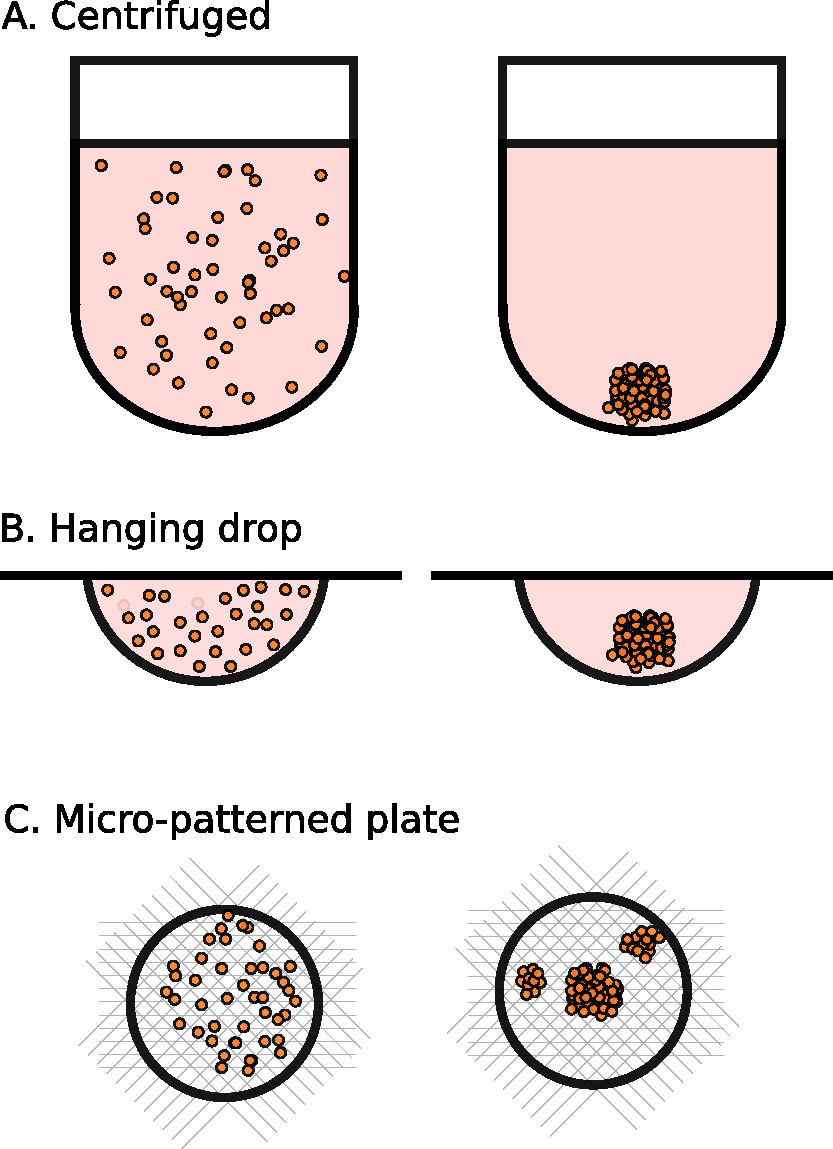
\includegraphics[width=0.3\textwidth]{ch4spheroidDiagram}
    \label{figure:spheroid_diagram}
\end{figure}

Despite the rapid adoption of 3D cellular models there is a lack of definitive evidence for their benefit over the more 
simple 2D models, in turn there are a number of additional issues which have to be addressed when using 3D tumour 
spheroids in an image-based assay.
Cells located within the centre of the spheroid are often difficult to image and in turn segment due to limited 
penetration depth of light sources and poor labelling of fluorescent reagents.
A number of commercially available high-throughput confocal microscopes are available which go some way to countering 
this issue, although to obtain adequate optical quality for single-cell segmentation usually requires chemical clearing 
methods.
Assuming sufficient clarity of fluorescently labelled cells throughout the depth of a spheroid there is a choice of 
using the 3D data for segmentation and analysis, or to project the 3D structure onto a 2D plane using maximum 
projection or another similar algorithm and process the image using standard 2D segmentation and image analysis tools.
While 3D data does offer a greater number of measurements through volumetric analysis and therefore a greater amount of 
morphological information, many researchers still opt for 2D image analysis of tumour spheroids owing to familiarity, 
the reduced computational resources required for storage and analysis, and the greater availability of established 
software tools.


\subsection{Proteomics to interrogate hits from high-content screening}
Interrogating hits found from target-agnostic phenotypic screens is often viewed as an important step to gain 
mechanistic information as well as generating hypotheses for new targets and disease aetiology.
Methods such as thermostability shift assays, microarrays, RNAseq, whole-genome CRISPR knockouts and quantitative mass 
spec all have various strengths and weaknesses which make them appropriate for certain experimental questions.
However, these methods are limited by either their focus on a single protein or by their limited throughput -- mainly 
due to high costs -- allowing analysis of only a small number of samples.

RPPA (Reverse Phase Protein microArray) is a miniaturised high-throughput antibody-based method for measuring abundance 
of total protein or translationally modified epitopes across a large number of samples.
Protein lysates are spotted onto a solid substrate in multiple arrays which are then individually probed in parallel 
with mono-specific antibodies conjugated to a fluorophore, protein abundance is then measured by comparing fluorescent 
signal against a dilution series of a known standard. \cite{Akbani2014}
One of the main benefits of RPPA over other methods is the ability to process a large number of samples in parallel, 
which can be used to profile a number of treatment conditions, time-points, or concentrations.
In contrast, the main limitation of RPPA is the reliance on high quality specific antibodies, which confines the 
detectable proteins and epitopes to those with well-validated and commercially available antibodies.
RPPA has a number of advantages over other proteomic techniques such as high-sensitivity, high sample capacity and low 
sample consumption which makes it a well suited tool to investigate hits resulting from a target-agnostic high-content 
screen.


\subsection{Screening approved drugs: repurposing old compounds}

Repurposing an existing drug to treat a new disease or indication is an attractive strategy for cost-effective drug 
discovery programmes.
Existing drugs have already been through pre-clinical and clinical safety studies, clinical trials and regulatory 
approval for their original indication and so the path from \textit{in vitro} and \textit{in vivo} screening to 
clinical use can be expedited and development costs greatly reduced.
These advantages have resulted in a number of pharmaceutical companies investing time and resources into looking for 
new opportunities to reposition their existing compounds while still under-patent, as well as a number of new biotech 
companies hoping to re-patent old drugs under a new method of use.

Using knowledge of an existing drugs mechanism on known targets to treat other diseases which share similar molecular 
targets is a simple strategy for drug repurposing.
One example is duloxetine, a serotonin and adrenergic reuptake inhibitor originally developed for the treatment of 
depression, which was later repositioned as an anti-incontinence therapy. \cite{Ashburn2004}
Serotonin and noradrenaline while well known for their effects on mood and behaviour, also produce an excitatory effect 
in smooth muscle neurons which can lead to an improvement in bladder control.
This was noted by Eli Lilly who now have approval to market duloxetine as both an anti-depressant as well as the first 
approved urinary incontinence medication.

Another approach to drug repurposing is to take advantage of so-called ``off-target'' effects.
The non-specific binding to other protein targets can be leveraged for unrelated diseases; an example of this is 
itraconazole, a broad spectrum anti-biotic which has been found to act through the Hedgehog pathway as a potential 
anti-cancer therapy. \cite{Pounds2017}


\subsection{Chapter aims}
The aim of this work was to screen a library of approved small molecules across a panel of eight breast cancer 
cell-lines to identify compounds which cause a distinct phenotypic response in one or more cell-lines.
Then to investigate these compounds using functional 2D and 3D tumour spheroid assays of cell death and viability and 
to highlight potential pathways responsible for their selective breast cancer cell-line response using RPPA to measure 
the abundance of 60 proteins representative of canonical cell survival and cell proliferation signalling pathways.



\section{Results}

\subsection{High-content screen of 1280 approved compounds}

The Prestwick library of 1280 approved compounds was used in a high-content image based screen at a single 1 $\mu$M 
concentration across all eight breast cancer cell-lines (table \ref{table:cell-lines}).
Multiple morphological features were quantified from the images using Cellprofiler image analysis software and 
aggregated to an image median, and normalised to the plate negative control values and standardised.
Plotting the first two principal components of this data revealed a clear separation between the positive (300 mM 
staurosporine) and negative control (0.1 \% DMSO) (figure \ref{figure:pca_early} A)
with a multivariate Z-factor\cite{Kummel2010} of 0.6 for the pooled cell-lines, and greater than 0.7 for individual 
cell-lines (table \ref{table:z_factors}) demonstrating a robust screening assay.
In addition, the data from the morphologically distinct cell-lines was mixed and not separately clustered (figure 
\ref{figure:pca_early} B), indicating that the normalisation step successfully removed basal cell-line morphologies 
enabling comparison of phenotypic response between morphologically distinct cell-lines.

\begin{figure}
    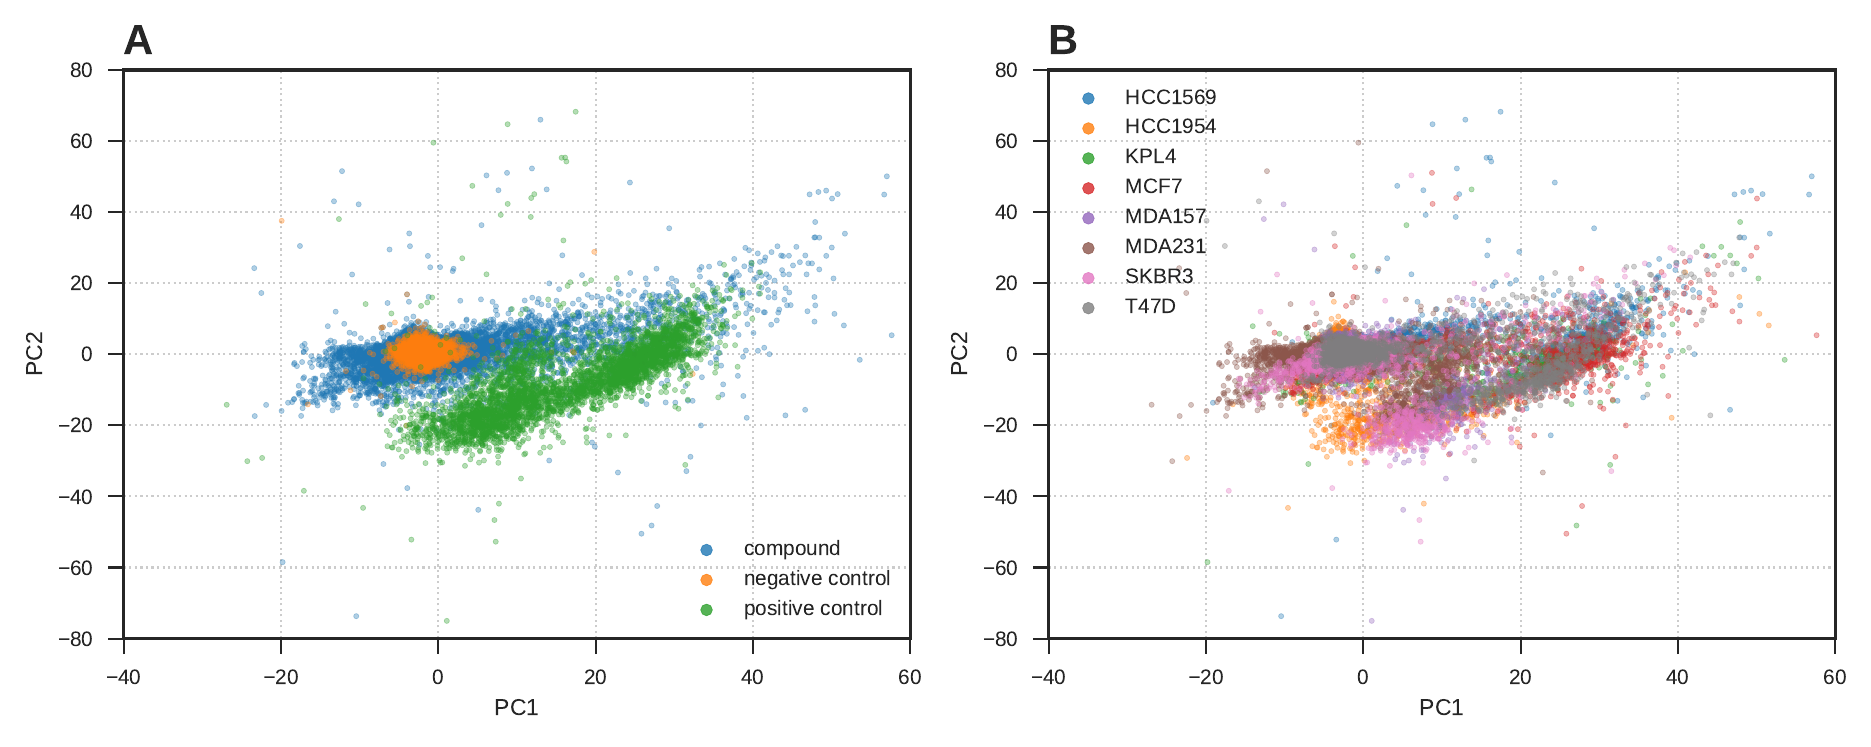
\includegraphics[width=1.05\textwidth]{ch4PCAearly.png}
    \captionsetup{width=0.8\textwidth}
    \caption[Principal components of the Prestwick approved compound library after normalisation and standardisation.]{
        Principal component analysis of the Prestwick approved compound library after normalisation and feature 
standardisation.
        Points represent individual images.
        \textbf{(A)} Data points colour coded drug treatment, positive control (300 nM staurosporine) or negative 
control (0.1 \% DMSO).
        \textbf{(B)} Data points colour coded by cell-line.
    }
    \label{figure:pca_early}
\end{figure}


\begin{table}[]
    \captionsetup{width=0.8\textwidth}
    \caption[Z-factor values of assay quality for each cell-line] {
        Multivariate Z-factor values of assay quality showing separation between the positive and negative control per 
cell-line.
    }
    \begin{footnotesize}
\begin{tabular}{@{}ll@{}}
    \toprule
    Cell line  & Z-factor \\ \midrule
    HCC1569    & 0.72     \\
    HCC1954    & 0.77     \\
    KPL4       & 0.84     \\
    MCF7       & 0.77     \\
    MDA-MB-157 & 0.78     \\
    MDA-MB-231 & 0.74     \\
    SKBR3      & 0.79     \\
    T47D       & 0.79     \\ \bottomrule
\end{tabular}
\end{footnotesize}
\label{table:z_factors}
\end{table}


\begin{table}
    \captionsetup{width=0.8\textwidth}
    \caption[Number of active compounds in the Prestwick library per cell-line]{
    Number of active compounds in the Prestwick library per cell-line.
    Compounds were defined as phenotypically active by calculating the $l_1$ norm distance from the negative control 
centroid in the principal components of the morphological features.
    }
    \begin{footnotesize}
\begin{tabular}{@{}ll@{}}
\toprule
Cell line  & \# active compounds \\ \midrule
HCC1569    & 283                 \\
HCC1954    & 182                 \\
KPL4       & 236                 \\
MCF7       & 287                 \\
MDA-MB-157 & 96                  \\
MDA-MB-231 & 352                 \\
SKBR3      & 218                 \\
T47D       & 327                 \\ \bottomrule
\end{tabular}
\end{footnotesize}
\label{table:active_per_cell_line}
\end{table}


For each phenotypically active compound in the Prestwick library the difference in response between pairs of cell-lines 
was measured using the TCCS method (chapter \ref{chapter:tccs}), and compound-cell-line-pairs were ranked in terms of 
decreasing $\Delta\theta$ values.
Compounds which demonstrated distinct phenotypic response were triaged by replication studies to confirm activity and 
selecting those with interesting MoAs for further studies as well as removing several microtubule disruptors.
Twelve hits were selected for further study (table \ref{table:hit_list}) based on phenotypic activity as determined 
with the $l_1$ norm from the negative control in principal component space, and rank by their ability to induce 
distinct phenotypic responses between the cell-lines measured with the TCCS method.
Selected compounds were repeated in triplicate, and ranked by $\Delta\theta$ value for each replication, and used to 
calculate a rank product to rank overall distinct phenotypic effects between cell-lines (table 
\ref{table:rank_products} shows the top 15 compound-cell-line pairs).

\begin{table}
    \captionsetup{width=0.8\textwidth}
    \caption[Table of initial hits from the Prestwick library which produced distinct phenotypic response between 
cell-lines.]{
        Table of hits selected from the Prestwick library which produced distinct phenotypic responses between 
cell-lines. SERT: serotonin reuptake transporter, SSRI: selective serotonin reuptake inhibitor, 5-HT: 
5-hydroxytryptamine, D$_{1/2}$ dopamine receptor.
    }
    \begin{footnotesize}
    \begin{tabular}{@{}ll@{}}
    \toprule
    Compound        & Usage / MoA                                     \\ \midrule
    Amodiaquine     & Anti-malarial.                                  \\
    Cisapride       & 5-HT$_4$ agonist                                \\
    Dilazep         & Vasodilator. Adenosine reuptake inhibitor       \\
    Fluvoxamine     & Anti-depressant. SSRI                           \\
    Ivermectin      & Anti-helmintic. GluCl agonist                   \\
    Niclosamide     & Anti-helmintic                                  \\
    Paroxetine      & Anti-depressant. SSRI                           \\ 
    Pirenperone     & 5-HT$_{2A}$ antagonist                          \\
    Podophyllotoxin & Microtubule destabiliser                        \\
    Protriptyline   & Tricyclic anti-depressant. NA, SERT             \\
    Triflupromazine & Antipsychotic. D$_1$, D$_2$ antagonist          \\
    Zalcitabine     & nucleoside reverse transcriptase inhibitor      \\ \bottomrule
    \end{tabular}
    \end{footnotesize}
    \label{table:hit_list}
\end{table}


\begin{table}[]
    \captionsetup{width=0.8\textwidth}
    \caption[Rank products of top 15 Prestwick hits followed up in triplicate]{
    Table showing the 12 selected Prestwick compounds repeated in triplicate, which were ranked by decreasing 
difference in phenotypic response between cell-lines and used to calculate a rank product.
    Table shows the top 15 out of 266 compound-cell-line pairs when ranked by increasing rank product.
    MDA231: MDA-MB-231. MDA157: MDA-MB-157.
    }
\begin{footnotesize}
\begin{tabular}{@{}lllll@{}}
\toprule
Cell line A & Cell line B & Compound        & Rank product & \% False positive \\ \midrule
HCC1569     & MDA231      & Podophyllotoxin & 7.01         & $3.88e^{-4}$      \\
KPL4        & MDA231      & Podophyllotoxin & 9.06         & $4.66e^{-4}$      \\
MDA231      & SKBR3       & Podophyllotoxin & 12.11        & $8.54e^{-4}$      \\
HCC1569     & HCC1954     & Fluvoxamine     & 12.22        & $6.31e^{-4}$      \\
HCC1569     & SKBR3       & Ivermectin      & 13.16        & $6.57e^{-4}$      \\
HCC1569     & HCC1954     & Triflupromazine & 13.66        & $6.28e^{-4}$      \\
HCC1954     & MCF7        & Ivermectin      & 16.54        & $9.52e^{-4}$      \\
HCC1954     & SKBR3       & Protriptyline   & 22.04        & $1.90e^{-3}$      \\
HCC1569     & MDA231      & Cisapride       & 22.10        & $1.73e^{-3}$      \\
HCC1954     & SKBR3       & Fluvoxamine     & 23.37        & $1.81e^{-3}$      \\
HCC1954     & T47D        & Triflupromazine & 23.49        & $1.68e^{-3}$      \\
MDA231      & T47D        & Cisapride       & 25.34        & $1.88e^{-3}$      \\
HCC1569     & MDA157      & Zalcitabine     & 25.96        & $1.88e^{-3}$      \\
HCC1954     & T47D        & Protriptyline   & 26.14        & $1.76e^{-3}$      \\ \bottomrule
\end{tabular}
\end{footnotesize}
\label{table:rank_products}
\end{table}


\subsection{Validation in 2D and 3D apoptotic assays}

\subsubsection{2D}

Using GFP expressing cell-lines with DRAQ7 as a marker of cell-death I performed concentration-response experiments 
with the 12 selected compounds.
Viable cells expressed nuclear GFP which was used as a simple readout of cell number, although the DRAQ7 apoptotic 
marker -- which fluoresces when bound to DNA but does not penetrate intact cell membranes -- did not provide robust or 
consistent data, as DRAQ7 positive apoptotic cells fluoresced only briefly before detaching from the bottom of the well 
and drifting out of the plane of focus (figure \ref{figure:incucyte_example}).
Therefore cell count using the GFP labelled nuclei was instead used as the readout in the concentration response 
experiment.

\begin{figure}[H]
    \fcapsideright{
    \caption[Example images of GFP and DRAQ7 T47D cells imaged with the incucyte]{
        Representative cropped images from the incucyte. GFP-labelled (green) T47D cells with DRAQ7 apoptotic marker 
(red) and phase contrast image (grey). Whole images from which these are cropped measure 2.15 mm$^2$.
        \textbf{(Left)} 0.1\% DMSO negative control cells.
        \textbf{(Right)} 0.3 $\mu$M staurosporine positive control.
    }
    } {
    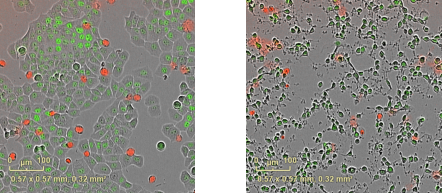
\includegraphics[scale=1.0]{ch4incucyteExample}
    \label{figure:incucyte_example}
    }
\end{figure}

Using 8 semi-log concentrations ranging from 0.3 nM to 1 $\mu$M and GFP cell-count normalised to the DMSO negative 
control as a measure of cell-viability, concentration response curves were plotted for the 12 compounds and 8 
cell-lines at the 72 hour time point (figure \ref{figure:2D_dose_response}).
Despite a selection criteria aiming to limit overtly cytotoxic compounds, 11 out of the 12 compounds demonstrated some 
form of concentration dependent reduction in cell-count in at least one of the cell-lines.
Zalcitabine was an exception with very little reduction in cell count, although at 1 $\mu$M concentration there was 
some evidence of reduced cell-count in MDA-MB-157 and HCC1569 cell-lines.
The HCC1569 cell-line demonstrated the greatest sensitivity to the majority of the tested compounds, especially to 
protryptyline which at 1 $\mu$M effectively killed all cells whilst largely unaffecting the 7 other breast cancer 
cell-lines.
Podophyllotoxin proved to be especially potent, with a relative cell-count below 50\% at the lowest tested 
concentration of 0.3 nM in 5 of the cell-lines.

\begin{figure}
    \includegraphics[width=1.0\textwidth]{ch42Ddoseresponse}
    \captionsetup{width=0.8\textwidth}
    \caption[Concentration-response curves for 12 hits from the Prestwick library in a 2D apoptosis assay.]{
        Concentration-response curves for 12 hits from the Prestwick library.
        Compounds were used in a 2D viability assay measuring cell count expressed as the percentage of the DMSO 
control after 72 hours.
    }
    \label{figure:2D_dose_response}
\end{figure}



\subsubsection{3D spheroid models}

A more complex 3D tumour spheroid assay was used to determine the functional effects of the 12 selected compounds in a 
more physiologically relevant environment.
All eight cell-lines were found to form consistent spheroids using the aggregation through centrifugation method and 
spheroid sizes with diameters around 500 $\mu$m.
Mirroring the 2D assay, GFP labelled cell-lines were used alongside DRAQ7 to measure cell viability and cell death, 
although in the case of spheroids the DRAQ7 staining was more consistent as DRAQ7-positive apoptotic cells remained 
aggregated in the spheroid in the focal plane (figure \ref{figure:spheroid_example}).
Spheroid area proved to be a poor readout for cell viability as cytotoxic treatment caused the spherical structure to 
collapse and disaggregate and so when imaged in 2D from above spheroid collapse results in an increase in measured 
spheroid area.
When increasing doses of cytotoxic compound were tested on spheroid this resulted in a paradoxical increase in spheroid 
area, even in the GFP channel as some residual GFP staining remained despite cell-death.
A measure of integrated intensity however proved a more intuitive readout of cell death within 3D spheroids and a 
comparison between the GFP and DRAQ7 channels revealed that the integrated intensity of GFP was more consistent and 
produced more robust concentration responses with staurosporine.

\begin{figure}
    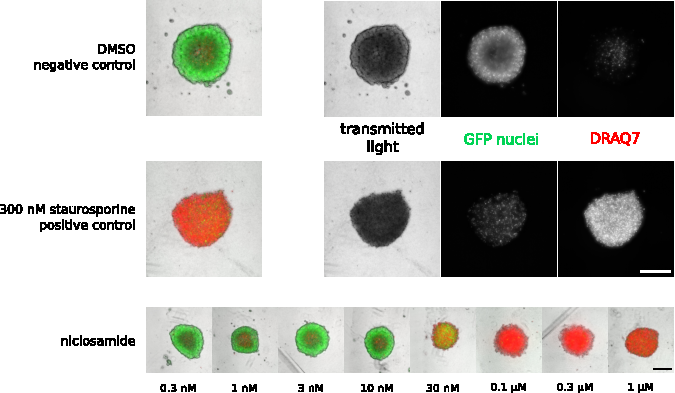
\includegraphics[width=0.8\textwidth]{ch4spheroidExample}
    \captionsetup{width=0.8\textwidth}
    \caption[Example images of T47D tumour spheroids.]{Example images of T47D tumour spheroids as imaged on the 
ImageXpress using transmitted light (grey), FITC (green) and CY5 (red) filters to visualise spheroid morphology. Scale 
bar = 300 $\mu$m}
    \label{figure:spheroid_example}
\end{figure}

Concentration response studies in 3D tumour spheroids with the 12 hits from the Prestwick library at 0.3 nM to 1 $\mu$M 
in semi-log concentrations after 72 hours revealed a decrease in sensitivity to the compounds compared to results 
obtained in the 2D assay (figure \ref{figure:3D_dose_response}).
Of the compounds which produced a concentration dependent response in 3D, most only elicited a decrease in GFP 
integrated intensity at the maximum 1 $\mu$M concentration tested.
The increased sensitivity of the HCC1569 cell-line compared to the others tested was not observed in 3D.
Of the 12 compounds tested podophyllotoxin and niclosamide produced robust sigmoidal concentration response curves, 
although not in all of the cell-lines.

\begin{figure}
    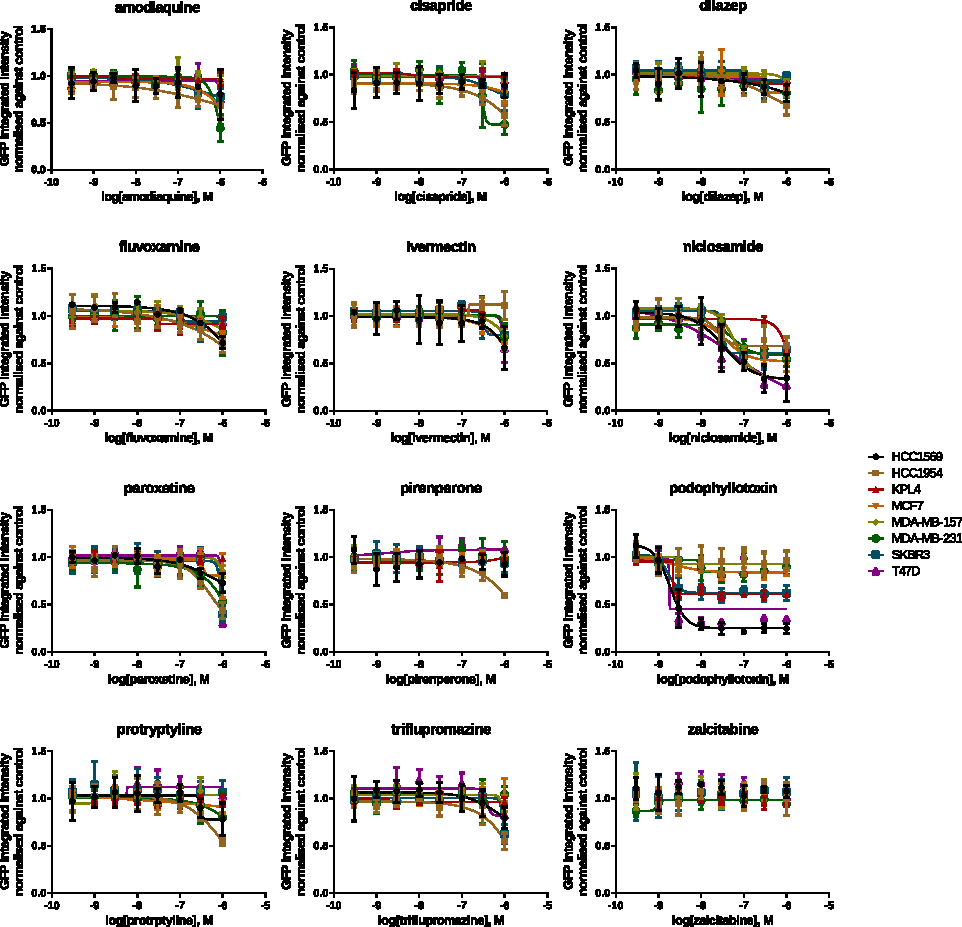
\includegraphics[width=1.0\textwidth]{ch43Ddoseresponse}
    \captionsetup{width=0.8\textwidth}
    \caption[Concentration-response curves for 12 hits from the Prestwick library.]{
        Concentration-response curves for 12 hits from the Prestwick library.
        Compounds were used in a 3D tumour spheroid viability assay measuring integrated intensity of GFP-labelled 
nuclei after 72 hours of compound treatment normalised against the negative control.
    }
    \label{figure:3D_dose_response}
\end{figure}


\subsection{RPPA}

Three compounds (ivermectin, protryptyline and niclosamide) were selected from the initial hit list based on their 
reproducibility and distinct response between cell-lines in both the morphological and viability assays.
These compounds were used in a proteomic study, in which the 8 breast cancer cell-lines were grown in 2D or 3D culture 
conditions and treated with 100 nM of compound for 72 hours, after which cells were lysed and RPPA was used to measure 
the abundance of 60 proteins and phosphoproteins.
Of the 60 proteins and phosphoproteins analysed 13 were discounted due to poor quality data such as low-signal to 
noise, poor spot morphology of samples printed on the RPPA chip and non-homogeneous or non-specific binding of 
antibodies to sample and/or chip -- leaving 47 measurements per sample.


\subsubsection{Cell-line and growth environment has a greater effect on protein expression than compound treatment}


These results show that the 3 active compounds (ivermectin, niclosamide and protryptyline) selected for RPPA analysis 
produce similar pathway response within in each cell-line.
However, compound induced pathway response diverge between distinct cell-lines and between 2D and 3D cell culture 
conditions.
Using the readout from the 47 measured epitopes, the 64 samples displayed obvious clustering according to cell-line in 
hierarchical clustering and projecting the data into 2 dimensions (figure \ref{figure:rppa_global_1} A,B,C).
Within the cell-line clusters there were distinct sub-clusters showing clear separation in the protein expression 
profiles of the two environmental conditions (figure \ref{figure:rppa_global_1} D).
Interestingly, growth environment (2D versus 3D culture conditions) produced a more distinct change in protein 
expression profile than compound treatment at 100 nM (figure \ref{figure:rppa_global_1} E).


\begin{figure}
    \includegraphics[width=1\textwidth]{ch4RPPAglobal1}
    \captionsetup{width=0.8\textwidth}
    \caption[Hierarchical clustering of RPPA samples.]{
        Globally normalised abundance of 64 samples, consisting of 8 cell-lines, 4 treatments and 2 growth conditions, 
measuring abundance of 47 proteins and phosphoproteins with RPPA.
        \textbf{(A)} Hierarchical clustering of protein samples from cells grown in 2D culture.
        \textbf{(B)} Hierarchical clustering of protein samples from cells grown in 3D spheroids.
        \textbf{(C)} Embedding of protein samples colour coded by cell-line.
        \textbf{(D)} Embedding of protein samples colour coded by environment conditions, either 2D culture of 3D 
tumour spheroids.
        \textbf{(E)} Embedding of protein samples colour coded by drug treatment.
    }
    \label{figure:rppa_global_1}
\end{figure}


\begin{figure}
    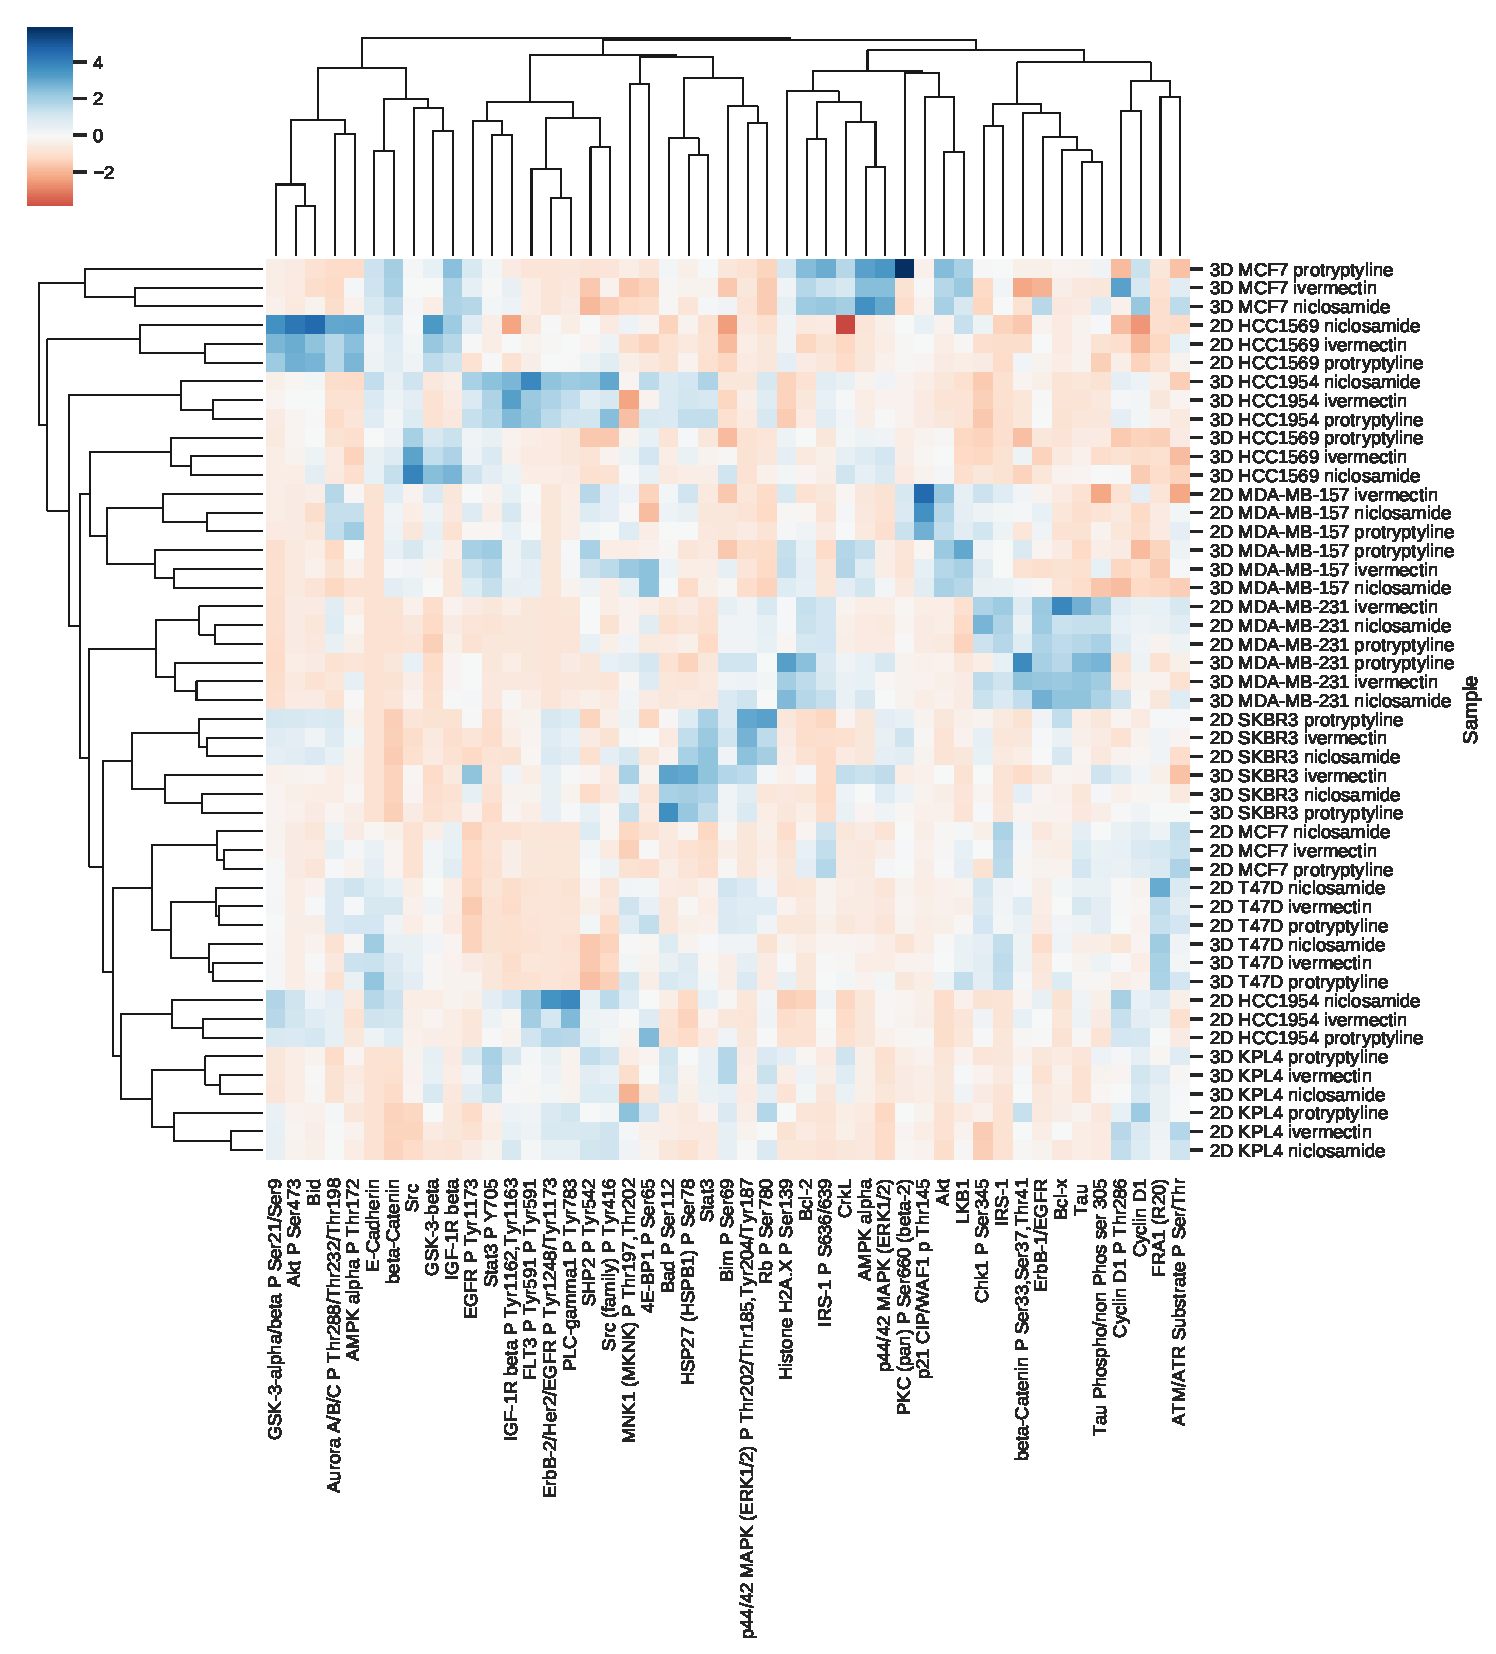
\includegraphics[width=1\textwidth]{ch4RPPAheatmap}
    \captionsetup{width=0.8\textwidth}
    \caption[Heatmap and clustering of RPPA data]{
        Heatmap of hierarchical clustering of globally normalised protein expression across cell-lines, growth 
environments and compound treatments.
    }
    \label{figure:rppa_heatmap}
\end{figure}


\subsubsection{Resistant cell lines treated with niclosamide or ivermectin show decreased expression of E-cadherin}

From the 2D concentration response studies it appeared that the cell-lines HCC1954 and SKBR3 both showed resistance to 
the anti-helmintic drugs niclosamide (figure \ref{figure:rppa_niclosamide_2D1} A) and ivermectin (figures 
\ref{figure:figure:rppa_ivermectin_2D} A)
By aggregating the sensitive (HCC1569, KPL4, MCF7, MDA-MB-157, MDA-MB-231, T47D) and insensitive (HCC1954 and SKBR3) 
RPPA data, it was possible to look at changes in protein expression shared among the differentially responding 
cell-lines.
Using data normalised to the DMSO control for each cell-line, and averaging the sensitive or insensitive cell-lines 
together revealed that both niclosamide and ivermectin treatment caused a distinct reduction of E-Cadherin in resistant 
cell-lines.
Cyclin D1 was another protein which was upregulated in the resistant cell-lines in response to both anti-helmintic 
treatments, which was not mirrored in sensitive cell-lines (figure \ref{figure:rppa_niclosamide_2D1} \% 
\ref{figure:rppa_ivermectin_2D} C\&D).


\begin{figure}
    \captionsetup{width=0.8\textwidth}
    \caption[Insensitivity of HCC1954 and SKBR3 to niclosamide in 2D]{
        Insensitivity of HCC1954 and SKBR3 to niclosamide in 2D.
        \textbf{(A)} Concentration response curve of normalised cell-count of 8 cell-lines treated with niclosamide (as 
shown in figure \ref{figure:2D_dose_response}).
        \textbf{(B\&C)} Mean change in protein abundance of cells grown in 2D treated with 100 nM drug compared to DMSO 
treated cells, averaged over multiple cell-lines.
        Y-axis indicates log$_2$ fold change from DMSO treated cells, error bars indicate $\pm$ standard deviation.
        }
    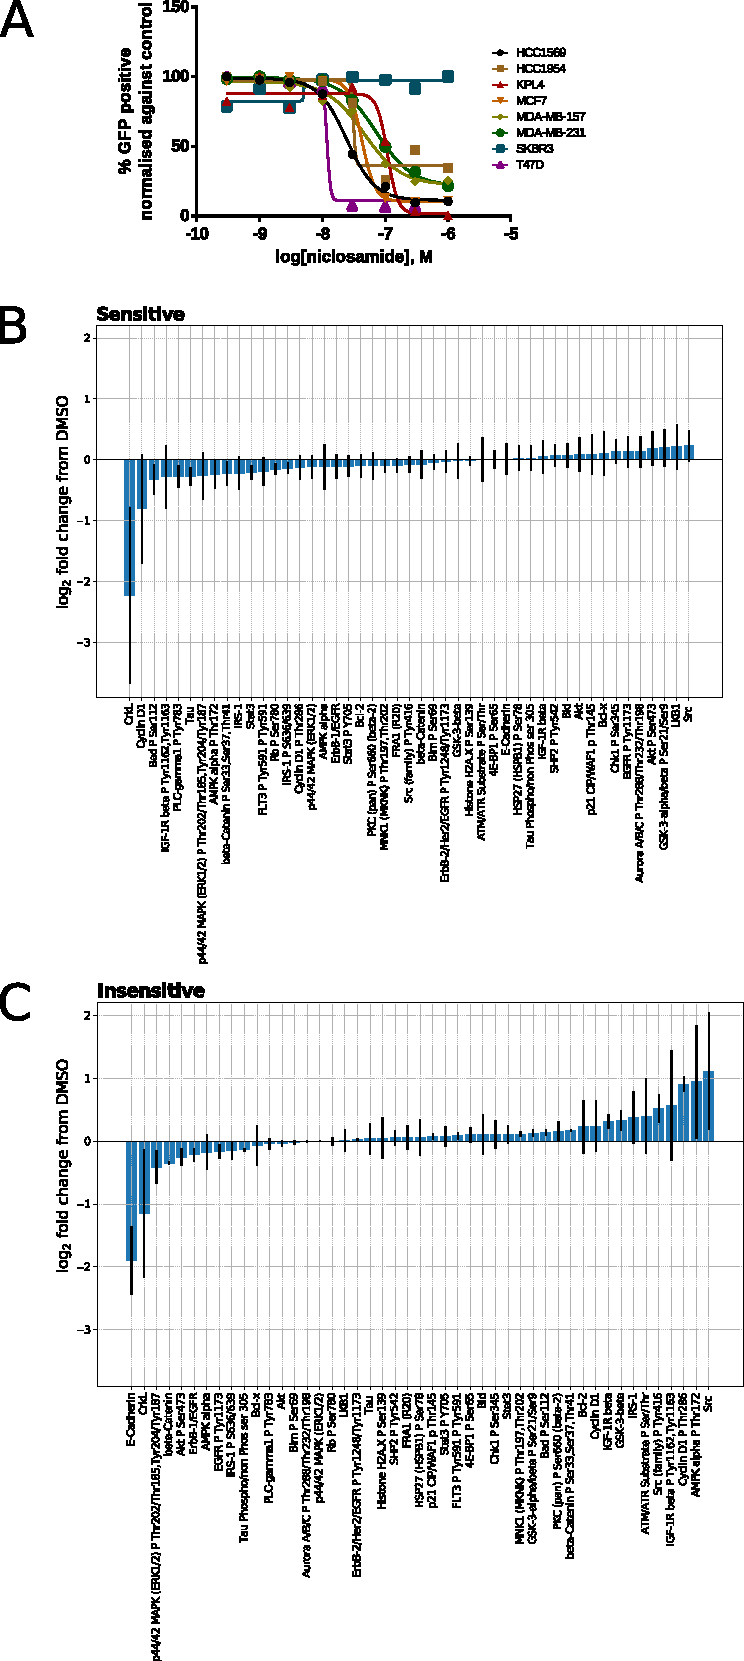
\includegraphics[width=0.7\textwidth]{ch4RPPAniclosamide2D1}
    \label{figure:rppa_niclosamide_2D1}
\end{figure}

\begin{figure}
    \captionsetup{width=0.8\textwidth}
    \caption[Insensitivity of HCC1954 and SKBR3 to ivermectin in 2D]{
        Insensitivity of HCC1954 and SKBR3 to ivermectin in 2D.
        \textbf{(A)} Concentration response curve of normalised cell-count of 8 cell-lines treated with ivermectin (as 
shown in figure \ref{figure:2D_dose_response}).
        \textbf{(B\&C)} Mean change in protein abundance of cells grown in 2D treated with 100 nM drug compared to DMSO 
treated cells, averaged over multiple cell-lines.
        Y-axis indicates log$_2$ fold change from DMSO treated cells, error bars indicate $\pm$ standard deviation.
        }
    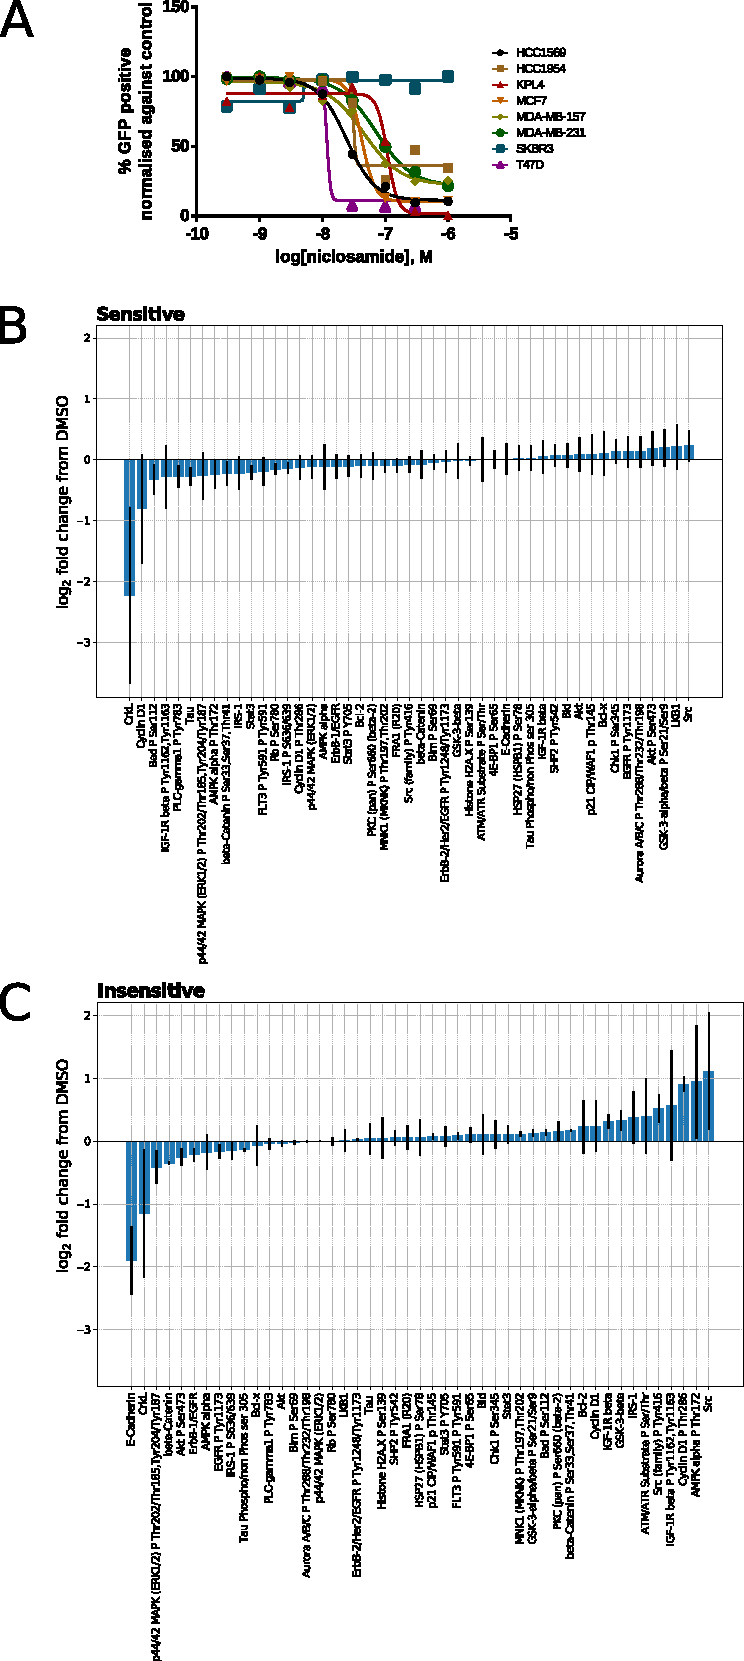
\includegraphics[width=0.7\textwidth]{ch4RPPAniclosamide2D1}
    \label{figure:rppa_ivermectin_2D}
\end{figure}

\subsubsection{Protryptyline shows different resistant cell-lines in 2D and 3D}
In the 2D concentration response assay HCC1569 demonstrated a singular sensitivity to the tricyclic antidepressant 
protryptyline (figure \ref{figure:rppa_protryptyline2D} A).
However, repeating the concentration response assay in 3D tumour spheroids ameliorated this sensitivity, and instead 
another cell-line -- HCC1954 -- showed a slight response to protryptyline which was not seen in the 7 other breast 
cancer cell-lines (figure \ref{figure:rppa_protryptyline3D} A).
RPPA data indicated that in 2D the sensitive HCC1569 cell-line had decreased levels of IGF-$\beta$ and MAPK 
phosphorylation compared to the resistant cell-lines (figure \ref{figure:rppa_protryptyline2D} B \& C), while in 3D the 
sensitive HCC1954 cell-line had a similar decrease in IGF-$\beta$ although a contradictory 2-fold increase in 
phosphorylated MAPK (figure \ref{figure:rppa_protryptyline3D} B).



\begin{figure}
    \captionsetup{width=0.8\textwidth}
    \caption[Sensitivities of cell-lines in 2D to protryptyline]{
    Sensitivities of cell-lines in 2D assays of cell viability, and corresponding changes in protein levels of 
sensitive and resistant groups.
    \textbf{(A)} Concentration response curve of integrated intensity of GFP expressing cell-lines treated with 
protryptyline in 2D cell-culture.
    \textbf{(B-C)} Mean changes in protein abundance of cells treated with 100 nM protryptyline. Y-axis indicates 
log$_2$ fold-change from DMSO treated cells, error bars indicate $\pm$ standard deviation.
    \textbf{(B)} RPPA data of the sensitive HCC1569 cell-line grown in 2D cell culture treated with protryptyline.
    \textbf{(C)} RPPA data of the 7 resistant cell-lines grown in 2D cell-culture treated with protryptyline.
        }
    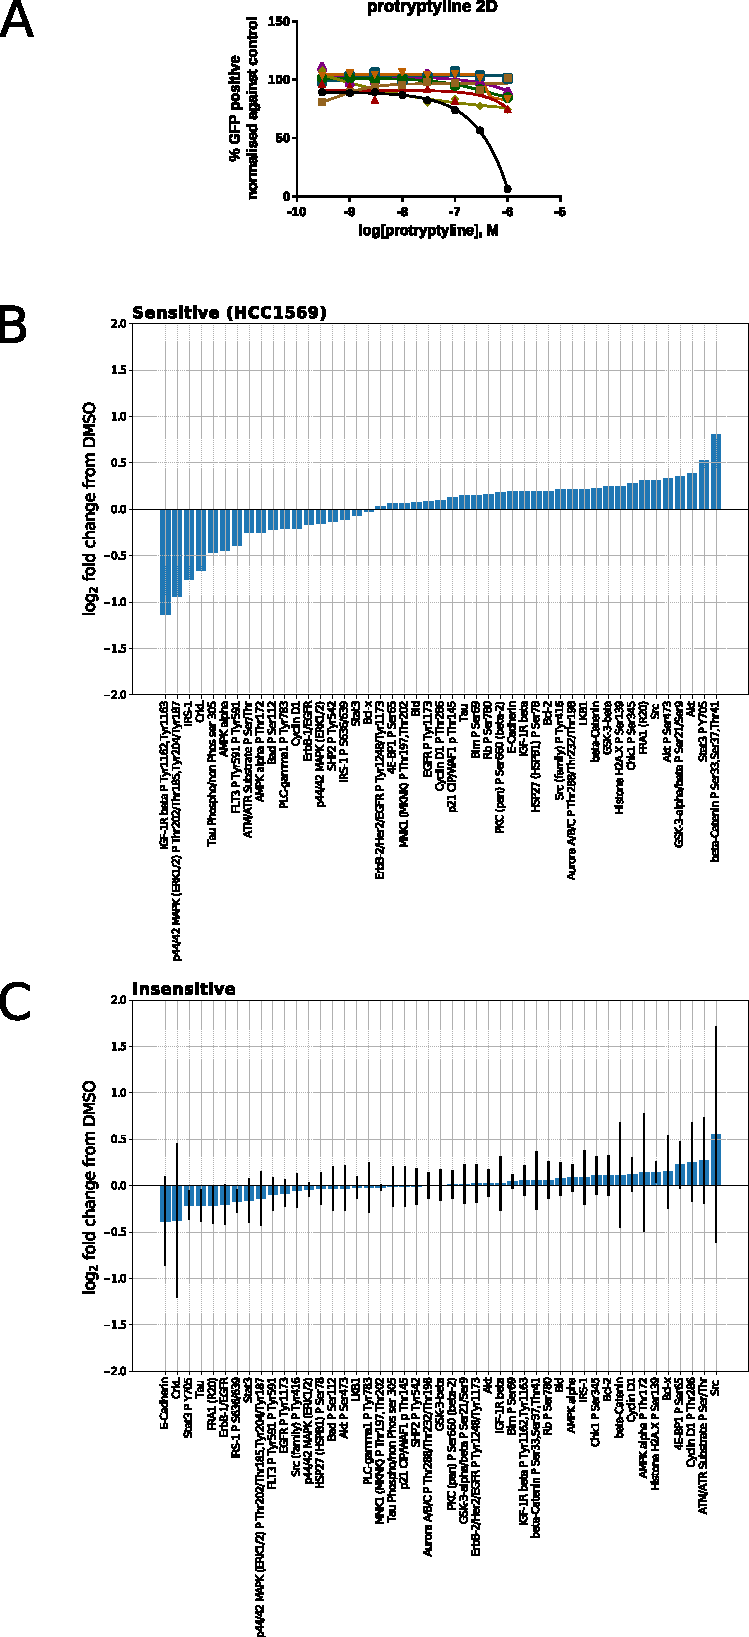
\includegraphics[width=0.7\textwidth]{ch4rppaProtryptyline2D}
    \label{figure:rppa_protryptyline2D}
\end{figure}


\begin{figure}
    \captionsetup{width=0.8\textwidth}
    \caption[Sensitivities of cell-lines in 3D to protryptyline]{
    Sensitivities of cell-lines in 3D assays of cell viability, and corresponding changes in protein levels of 
sensitive and resistant groups.
    \textbf{(A)} Concentration response curve of integrated intensity of GFP expressing cell-lines treated with 
protryptyline in 3D tumour spheroids.
    \textbf{(B-C)} Mean changes in protein abundance of cells treated with 100 nM protryptyline. Y-axis indicates 
log$_2$ fold-change from DMSO treated cells, error bars indicate $\pm$ standard deviation.
    \textbf{(B)} RPPA data of the sensitive HCC1954 cell-line grown in 3D spheroids treated with protryptyline.
    \textbf{(C)} RPPA data of the 7 resistant cell-lines grown in 3D spheroids treated with protryptyline.
        }
    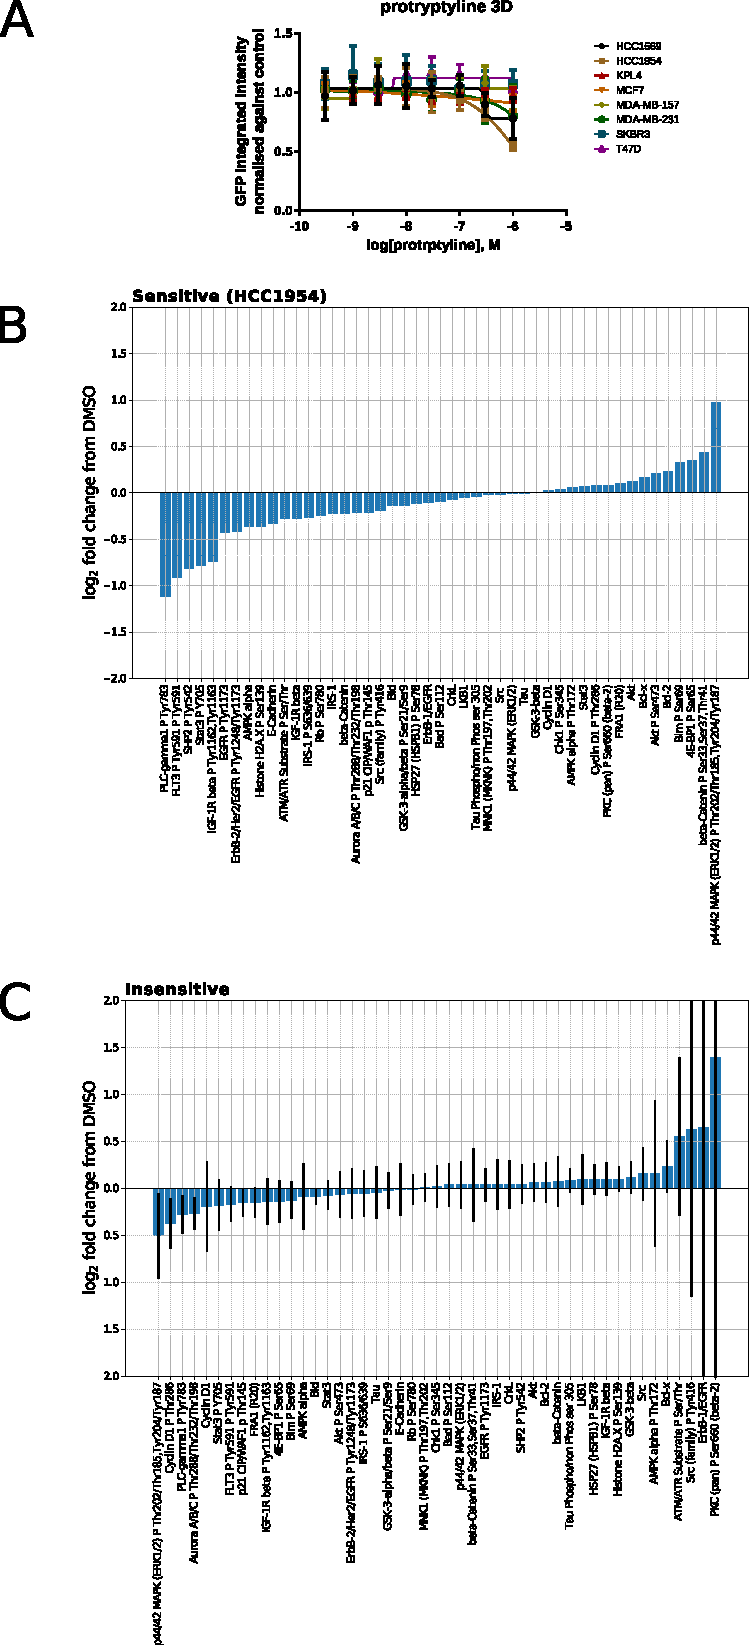
\includegraphics[width=0.7\textwidth]{ch4rppaProtryptyline3D}
    \label{figure:rppa_protryptyline3D}
\end{figure}


\subsubsection{Cells cultured in tumour spheroids have increased Src and decreased Aurora kinase phosphorylation}
Cells grown in 2D on tissue culture plastic are subjected to different environmental stimuli to those grown in 3D, with 
cell-to-cell adhesions, presence of extracellular matrix and differences in oxygen and nutrient supply all effecting 
intracellular signalling and therefore protein expression and response to external stimuli.
Using the RPPA data from the negative control treated samples grown in 2D and 3D revealed a number of proteins which 
had altered expression dependent on the environmental conditions.
In 3D conditions the phosphorylated form of Aurora A/B/C had a two-fold decrease over cells grown in 2D, while Src 
kinase and AMPK alpha showed a 2 and 4-fold increase respectively in cells grown in 3D compared to 2D (figure 
\ref{figure:rppa_2D_3D_diff}).
The decrease in phosphorylated aurora kinase in 3D spheroids may be indicative of the cell-cycle arrest commonly seen 
in cells located towards the centre of the spheroid. \cite{Laurent2013a}
For certain proteins such as AMPK alpha there is a large variation between the cell-lines and as there is only a single 
sample per condition it is not possible to determine if this is an inherent difference in the response to environmental 
conditions between the cell-lines or simply noise within the data.
The elevation of Src kinase in 3D spheroid cultures (figure \ref{figure:rppa_2D_3D_diff}) is potentially interesting in 
relation to the general decrease in drug sensitivity of hit compounds observed in 3D spheroid and 2D assays (figures 
\ref{figure:2D_dose_response} \& \ref{figure:3D_dose_response}).


\begin{figure}
    \captionsetup{width=0.8\textwidth}
    \caption[Difference in protein expression in cells grown in 3D compared to 2D]{
        Comparison of protein expression between cells grown in 3D or 2D environments.
        The median difference from combined data from 8 cell-lines treated with 0.1 \% DMSO.
        Difference is represented as the $\log_{2}$ fold change of 3D expression divided by 2D expression.
        Proteins with increased expression in 3D shown in blue, those with decreased expression in 3D relative to 2D 
shown in orange/red.
        Error bars indicate $\pm$ median absolute deviation of the 8 cell-lines.
    }
    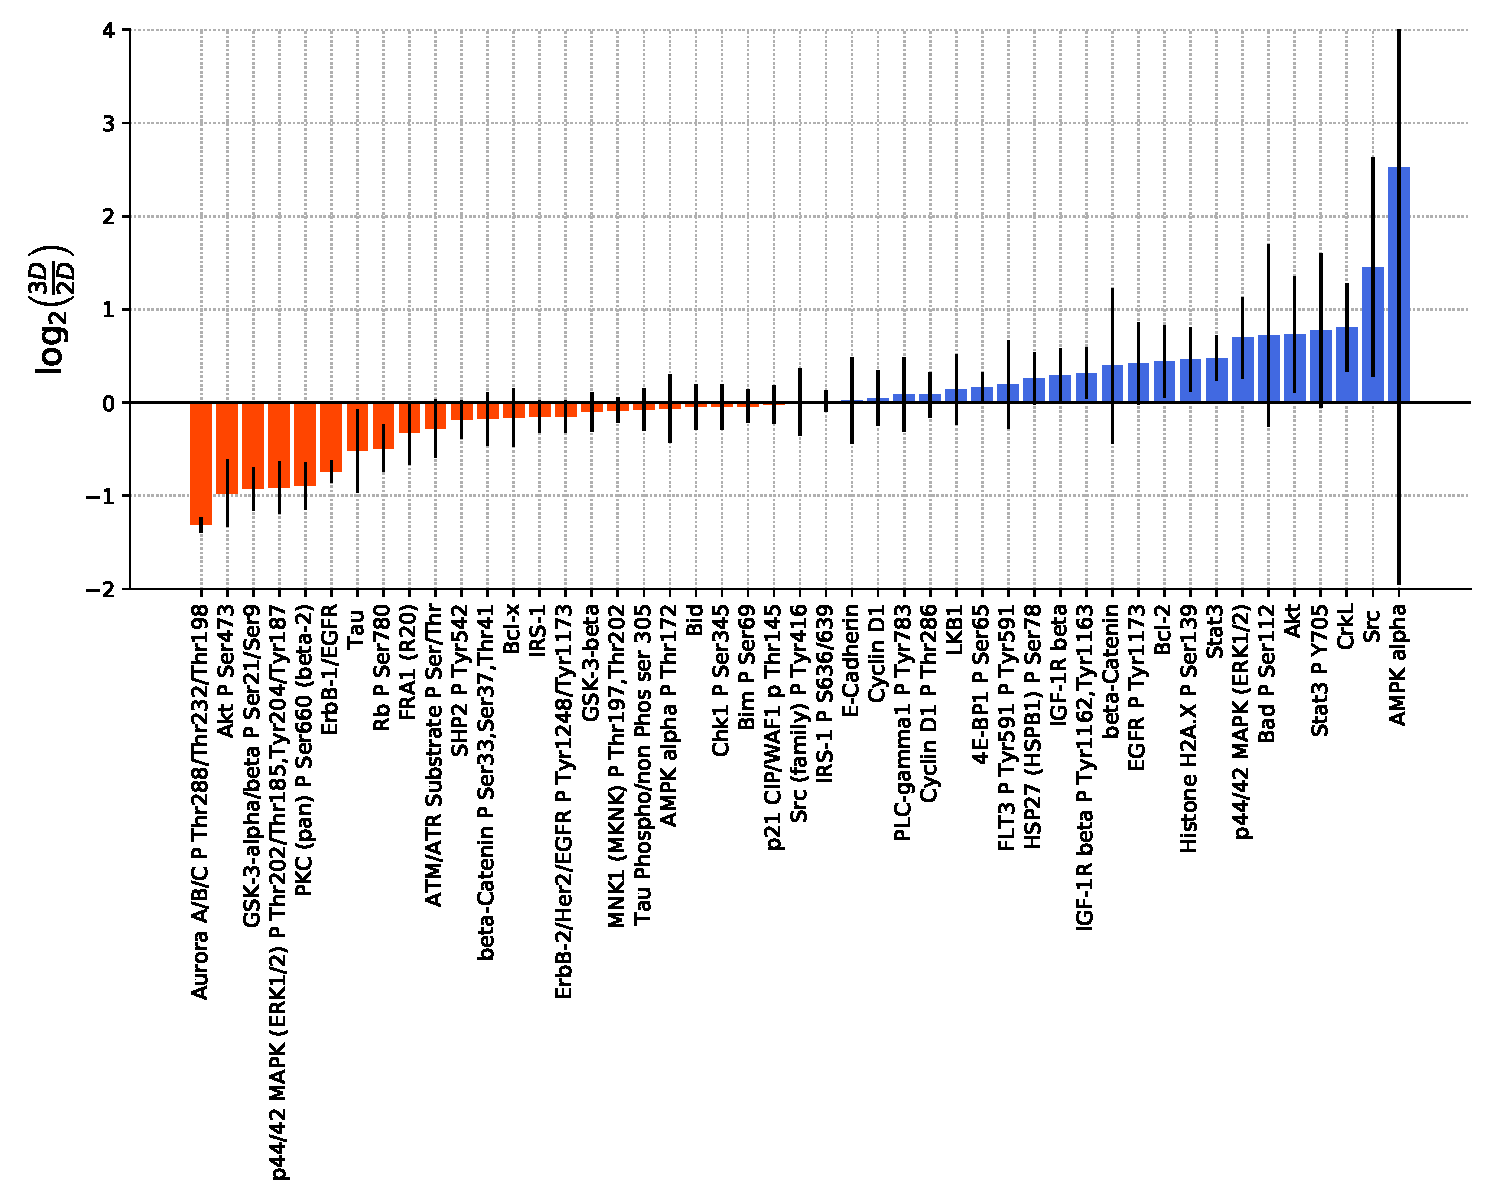
\includegraphics[width=0.8\textwidth]{ch42D3Ddiff}
    \label{figure:rppa_2D_3D_diff}
\end{figure}



\section{Discussion}

A number of approved compounds were identified with a high-content screen which resulted in distinct phenotypic 
responses between breast cancer cell-lines.
Following validation in 2D and 3D models of cell proliferation and survival, two anti-helmintic compounds (ivermectin 
and niclosamide) and a antidepressant (protryptyline) were selected for further investigation of their anti-cancer MoA.
Proteomic analysis of cells grown in 2D and 3D tumour spheroids treated with these compounds revealed that both 
anti-helmintic treatments caused a reduction in E-cadherin levels in resistant cell-lines which was not observed in the 
sensitive cell-lines.
Reduction in E-cadherin expression levels has previously been associated with epithelial-mesenchymal transition during 
tumour progression and the onset of more cancer stem-cell like phenotypic associated with drug resistance. 
\cite{Izumiya2012,Farmakovskaya2016}
Cyclin D1 was another protein upregulated in the resistant cell-lines in response to both anti-helmintic treatments.
Several studies have implicated elevated Cyclin D1 with drug resistance in part through a dual role in promoting cell 
proliferation and inhibition of drug-induced apoptosis. \cite{Biliran2005}
Previous transcriptomic studies have also shown that Cyclin D1 over-expression in tumours alters the expression of 
genes controlling cell metabolism and disrupt REDOX balance by producing reactive oxygen species and oxidative stress 
signalling pathways which influence drug sensitivity. \cite{Bustany2016}
It was also found that culturing tumour cells in complex 3D environments resulted in a number of changes in protein 
levels of cell-cycle regulators, which is in agreement with existing studies which have found reduced proliferation and 
cell-cycle arrest of many cells within the core of a spheroid.\cite{Laurent2013a}
The reduced proliferation of cells when cultured in tumour spheroids may also explain the reduced sensitivity of 
cell-lines in response to all test compounds when compared to those grown in 2D (figure \ref{figure:2D_dose_response} 
and \ref{figure:3D_dose_response}), as many cytotoxic compounds act through cell-cycle checkpoints or microtubule 
dynamics during cell-division.
In addition, RPPA analysis further revealed elevated levels of the non-receptor tyrosine kinase Src in 3D spheroid 
cultures which is associated with cancer cell survival signalling and a common pathway of drug resistance in breast 
cancer and other tumour types. \cite{Zhang2011a}

The approved compounds identified in this work which produce distinct morphological effects between different 
cell-lines may be a consequence of altered signalling pathways, differences in expression of target receptors or one of 
many other biologically interesting possibilities.
However, a simple explanation would be that the morphological differences observed are actually differences in 
sensitivity caused by multi-drug resistance efflux pumps.
Elevated expression of ATP binding cassette (ABC) drug efflux transporters are found in many types of cancer, and are 
suggested to contribute towards chemo-resistance in breast cancer. \cite{Kuo2007}
Considering certain cell-lines such as HCC1569 were commonly more sensitive to a number of the tested compounds (figure 
\ref{figure:2D_dose_response}), it would be worthwhile to determine if expression of multi-drug efflux pumps correlated 
with cell-line sensitivity and may explain a number of the distinct responses observed.

The majority of the hits found in this phenotypic screen (table \ref{table:hit_list}) have also been proposed as 
potential candidates for repurposing.
Amodiaquine originally developed as a selective anti-malarial treatment has been reported to have anti-adipogenic 
properties. \cite{Kim2017}
Multiple studies have proposed repurposing the anti-helmintic drugs ivermectin and niclosamide as potential anti-cancer 
treatments, \cite{Juarez2018,Wu2018} cisapride as a treatment for Chagas disease, \cite{Dietrich2018} dilazep to aid 
HIV treatment,\cite{Zeng2014} fluvoxamine as an inhibitor of glioblastoma invasion, \cite{Hayashi2016} protryptyline as 
a treatment for osteosarcoma, \cite{Su2016} paroxetine as a neuroprotective agent \cite{Steiner2015,Meulendyke2014} and 
podophyllotoxin and triflupromazine as anti-cancer treatments. \cite{Wu2018,Rigas1981}
A potential issue with the Prestwick chemical library screen performed in this study is the concentration at which the 
compounds are screened at.
The choice of which concentration to screen a compound library at is an open problem in the field, typically compound 
libraries consist of lead-like molecules which have not been optimised for potency -- which is not the case for many of 
the highly potent compounds found in the approved Prestwick library.
It may be a possibility that screening at 1 $\mu$M and discarding compounds which caused considerable toxicity has 
removed many potent and selective hits from the analysis, and screening at a lower concentration may have yielded a 
considerably different selection of hit compounds.
Similarly, performing RPPA analysis of pathway effects across concentration-response and time-series studies for each 
compound may reveal further insights into the pathways underpinning the anti-cancer activity than has been revealed by 
the single (100 nM) experiment performed in this project.

The functional assays used in this work are using cell-count (and integrated intensity of nuclei staining in the case 
of 3D models) as a surrogate measurement for cytotoxicity or cell-proliferation.
This functional readout is not ideal as the compounds chosen from the high-content screen were selected based 
preferentially on morphology measurements and their limited cytotoxicity.
The originally proposed functional assay was to test compound effect on the cell's ability to migrate through an 
extracellular matrix.
After trialling both 2D scratch wound assays through collagen and Matrigel substrates as well as 3D cell invasion assay 
from tumour spheroids embedded in extracellular matrix, I found that only the MDA-MB-231 cell-line was capable of 
migrating through collagen or Matrigel.
So while it would have been possible to confirm hits from the high-content screen in a single cell-line, it would not 
provide a comparison of functional activity between the cell-lines.

In summary the use of more complex cellular models to follow up hits resulting from a multiparametric high-content 
screen does offer an opportunity to gain an understanding of the functional affects of altered cellular morphology, 
however the choice of functional assay needs to be carefully considered to ensure it is relevant and robust.
Ideally a morphological change in simple 2D assay that is predictive of a functional response in a more complex and 
disease relevant 3D cell model offers an opportunity to combine large chemical libraries with more predictive and 
biologically relevant assays without the considerable cost burden associated with screening complex cell models at 
scale.




\section{Methods}

\subsection{Imaging and image analysis}
Cells were stained following the cell painting protocol, imaged with the ImageXpress and images were analysed with 
cellprofiler as previously described in the general methods (chapter \ref{chapter:generalMethods}).


\subsection{Compound library}
The compound library used was the Prestwick chemical library of 1280 off-patent small molecules, 95\% of which are 
approved drugs (FDA, EMA or others) stored as 10 mM stocks in DMSO.
For screening the library was assayed at a 1 $\mu$M final concentration.


\subsection{Multivariate Z-factor to determine assay quality}
A multivariate Z-factor as defined by Kümmel \textit{et al.}\cite{Kummel2010} is a multi-variate adaptation of the 
original Z-factor, \cite{Zhang1999} which is a measure of assay robustness in high-throughput screening.
The original measure is univariate, defined as:

\begin{equation}
    \text{Z-factor} = 1 - \frac{3(\sigma_p + \sigma_n)}
                               {|\mu_p - \mu_n|}
\end{equation}

where $\sigma_p$ and $\sigma_n$ are the standard deviations of the positive and negative control, and $\mu_p$ and 
$\mu_n$ the means of the positive and negative control.
A Z-factor of greater than 0.5 shows a very clear separation of positive and negative control, and is interpreted as an 
ideal assay.
The adaption of Kümmel \textit{et al.} uses linear discriminant analysis to find a combination of features to best 
separate the positive and negative controls, and calculates the Z-factor on the first linear discriminant.


\subsection{Identifying hits}

Hits were identified as those compounds which caused distinct phenotypic responses between cell-lines, excluding 
compounds which demonstrated significant toxicity.
This was first carried out by screening the entire 1280 compound library across the panel of eight cell-lines at 1 
$\mu$M concentration in 384-well optical bottomed plates (see chapter \ref{chapter:generalMethods}).
Following data pre-processing, distinct phenotypic responses between active compounds were calculated using the TCCS 
method (chapter \ref{chapter:tccs}).
An initial hit list was created by ranking compounds and cell-line pairs by decreasing $\Delta\theta$.
Compounds were triaged by removing those with less interesting mechanistic properties such as microtubule disruptors 
leaving 14 hits.
From these 14 hits, 2 were not easily available due to lack of a commercial supplier (pinaverium bromide) or being a 
controlled substance (3,4-dimethoxyphenethylamine).
The remaining 10 compounds were re-screened in triplicate at 8 semi-log concentrations ranging from 0.3 nM to 1 $\mu$M 
across the eight-cell lines to confirm a concentration-response relationship using the $l_1$ norm from the negative 
control as a measure of compound response.
Of those compounds that validated with a robust concentration dependent response $\Delta\theta$ values were calculated 
between all pairs of cell-line for each replicate dataset, and ranked by order of decreasing $\Delta\theta$, so that 
compounds-cell-line-pairs with a more distinct phenotypic response received a lower rank.
A rank product \cite{Breitling2004} was calculated from the replicates and compound-cell-line-pairs were sorted by 
increasing rank product.
Compounds that demonstrated repeatability and significantly low rank-products were carried onto more complex 2D and 3D 
apoptosis assays.


\subsubsection{Rank product}

A rank product algorithm with permutation-based significance testing was implemented in python.
Given a dataset of $k$ replicates and $n$ ranks, an $n$ by $k$ matrix with each row representing ranks from $[1..n]$.
For $[1..p]$ where $p$ is the number of permutations, the ranks in each row are shuffled and the geometric mean 
calculated for each column.
This yields a $p$ by $n$ matrix of permuted rank products which are used to count how many times the observed rank 
products from the replicated data is smaller than or equal to the permuted rank products, giving a value $c$.
The averaged expected value $E$ is then calculated as $E = p / c$ which is then used to calculate the percentage of 
false positives as $E$ divided by the rank of compound-cell-line-pair ordered by increasing rank-product value.


\subsection{2D apoptosis assay}

GFP-labelled cell-lines were seeded into the inner 60 wells of a flat-bottomed tissue culture treated 96-well plate 
(\#655180 Greiner), with approximately 10,000 cells per 90 $\mu$L of DMEM media, with the addition of 10 $\mu$L of 10\% 
DRAQ7 apoptotic marker (\#DR710HC biostatus), for a final DRAQ7 concentration of 3 $\mu$M.
Assay plates were then incubated at 37$^\circ$C, 5\% CO$_2$ incubator for 24 hours before addition of compounds.
Compounds were diluted in DMSO at 1000X concentration and assay plates were treated with the use of an intermediate 
plate as described in chapter \ref{chapter:generalMethods}.
Compound concentrations ranged from 0.3 nM to 1 $\mu$M with 0.1 \% DMSO as a negative control and 300 nM staurosporine 
as a positive control.
After compound treatments assay plates were then incubated for an additional 72 hours in the presence of compounds 
imaging with the incucyte ZOOM, imaging 3 sites per well in phase, red, and green channels every 3 hours.
Using the Incucyte ZOOM software, cells were counted in both the red and green channels for each site and timepoint and 
exported as csv files.
Data was merged with compound name and concentration data and filtered to select just the 72 hour time point.
Using the cell-count from the GFP channel, the count for each well then was expressed as a percentage of the median 
DMSO values per plate.
Concentration response-curves were fitted in GraphPad Prism (version 5) using a 4-parameter non-linear curve fit with 
least-squares.


\subsection{Spheroids}

\subsubsection{Creating spheroids}
Spheroids were created  by seeding approximately 10,000 GFP-expressing cells per well in 50 $\mu$L of media into each 
well of a 96-well ultra low attachment U-bottomed plate (\#7007 Corning).
A solution containing 4\% growth-factor reduced Matrigel (\#35623 Corning) and 2\% DRAQ7 apoptotic stain (\#DR710HC 
biostatus) was made in cold media, and 50 $\mu$L per well was added to the existing cell suspension, for a final 
Matrigel concentration of 2\% and 1\% DRAQ7.
Plates were then centrifuged for 10 minutes at 1000X G and 4$^\circ$ with brake speed reduced to pellet down the cells 
in the centre of each well.
After centrifugation plates were placed in a tissue culture incubator for 24 hours before addition of compounds.
Compounds from a 1000x source plate were diluted 1:50 by transferring 3 $\mu$L from the source plate to an intermediate 
plate containing 150 $\mu$L of media.
From the intermediate plate 5 $\mu$L were transferred to the spheroid assay plate containing 100 $\mu$L for a final 
dilution of 1:1000 and a DMSO concentration of 0.1\%.
Following compound addition spheroid plates were incubated for an additional 72 hours.


\subsubsection{Imaging spheroids}

Spheroids were imaged on the ImageXpress using the 4X objective lens in 3 channels (transmitted light, GFP and CY5).
Images were captured by first detecting the well-bottom in the centre of the U-bottomed well with a laser-based 
autofocus and offsetting by the well thickness, then capturing images in a z-stack at 8 focal planes spaced at 50 
$\mu$m intervals for a total range of 350 $\mu$m.
Z-stacks of the GFP and CY5 fluorescent channels were collapsed into a single image per channel using a maximum 
intensity projection, while the z-stack of transmitted light images were transformed using a minimum intensity 
projection.


\subsection{RPPA}

\subsubsection{Protein extraction}

\paragraph{2D cells.}
Protein extraction from 2D cells was performed by first seeding approximately 50,000 cells per well of a 6-well plates 
in 3 mL of media followed by incubation in a tissue culture incubator for 24 hours.
Compound addition was performed by diluting compound stocks in DMSO 1:50 in media to an intermediate plate, followed by 
1:20 from the intermediate plate to the assay plate for a 1000-fold dilution and 0.1\% DMSO.
Assay plates were then incubated for an additional 72 hours, after which wells were washed with 1 mL of room 
temperature PBS followed by addition of 100 $\mu$L of room temperature CLB1 (Zeptosens, Bayer) lysis buffer.
Cells and lysis buffer were then scraped into 1.5 mL eppendorf tube and incubated at room temperature for 30 minutes 
with frequent vortexing.
After 30 minutes of incubation lysis solution was centrifuged for 10 minutes at 13,000X G at room temperature and the 
supernatant was transferred into new 1.5 mL eppendorf tubes.

\paragraph{Spheroids.}
Protein extraction from spheroids was performed by first growing spheroids in 96-well plates following the same 
protocol as for imaging.
20 spheroids per treatment group were extracted with a pipette into a 1.5 mL eppendorf tube.
Pipette tips were widened by cutting with scissors.
The spheroids were then centrifuged for 30 seconds at 13,000X G at room temperature to pellet at the bottom of the 
tube, media was removed with a pipette and replaced with room temperature PBS.
Spheroids were pelleted again, PBS removed and replaced with 75 $\mu$L of room temperature CLB1 lysis buffer.
The spheroid lysis buffer mixture was incubated at room temperature for 30 minutes with frequent vortexing to break up 
cell aggregates.
Following incubation the lysis solution was centrifuged for 10 minutes at 13,000X G at room temperature, and 
supernatant extracted into a new 1.5 mL eppendorf tube.

\paragraph{Determining protein concentration.}
Protein concentration was determined with a Bradford assay, using a standard curve of known BSA concentrations and the 
addition of CLB1 lysis buffer to control for the lysis buffer concentration of the samples.
A curve of known BSA concentrations was created using 2 mg/mL BSA protein standard (\#23209 Thermo Scientific) diluted 
in PBS, with a 1:20 concentration of lysis buffer (see table \ref{table:bradford}).
Samples were diluted 1:20 in PBS by adding 2.5 $\mu$L of sample to 47.5 $\mu$L of PBS and mixed with a vortex.
10 $\mu$L of diluted samples and standard were added to each well of a flat-bottomed 96-well plate, followed by 240 
$\mu$L of room temperature Coomassie Plus Protein Assay (\#1856210 Thermo Scientific) and incubated at room temperature 
for 10 minutes.
Plates were then read with a microplate reader (BIORAD iMark) at a wavelength of 595 nm.
The protein concentrations of samples were calculated from a linear model of the BSA standard curve.
All protein samples were normalised to 1 mg/mL by dilution in CLB1 lysis buffer.

\begin{table}[h]
    \begin{footnotesize}
    \captionsetup{width=0.8\linewidth}
    \centering
        \caption[Bradford standard BSA curve]{
            Volumes for the BSA standard curve. Lysis buffer was CLB1, the same as used for the sample preparation.
        }
    \label{table:bradford}
    \begin{tabular}{@{}llll@{}}
        \toprule
        \begin{tabular}[c]{@{}l@{}}BSA final\\ concentration (mg/mL)\end{tabular} & \begin{tabular}[c]{@{}l@{}}BSA 2 
mg/mL\\ ($\mu$L)\end{tabular} & PBS ($\mu$L) & Lysis Buffer ($\mu$L) \\ \midrule
            0                                                                         & 0                               
                               & 95           & 5                     \\
            0.05                                                                      & 2.5                             
                               & 92.5         & 5                     \\
            0.1                                                                       & 5                               
                               & 90           & 5                     \\
            0.15                                                                      & 7.5                             
                               & 87.5         & 5                     \\
            0.2                                                                       & 10                              
                               & 85           & 5                     \\
            0.3                                                                       & 15                              
                               & 80           & 5                     \\
            0.4                                                                       & 20                              
                               & 75           & 5                     \\
            0.6                                                                       & 30                              
                               & 65           & 5                     \\ \bottomrule
    \end{tabular}
    \end{footnotesize}
\end{table}


\subsubsection{Zeptosens RPPA platform}

\textit{The RPPA study was performed on a Zeptosens platform by the Protein and Antibody Microarray facility at the 
Edinburgh Cancer Research UK Centre.}\footnote{A thank you to Alison Munro (University of Edinburgh) for running the 64 
samples on the Zeptosens RPPA platform.}

With the concentration-normalised protein lysates a final 4-fold concentration series of; 0.2; 0.15; 0.1 and 0.75 mg/mL 
in spotting buffer CSBL1 (Zeptosens-Bayer) was created.
The diluted concentration series of each sample was printed onto hydrophobic Zeptosens protein microarray chips 
(ZeptoChipTM, Zeptosens-Bayer) under environmentally controlled conditions (constant 50\% humidity and 14°C 
temperature) using a non-contact printer (Nanoplotter 2.1e, GeSiM).
A single 400 pL droplet of each lysate concentration was deposited onto the Zeptosens chip.
A reference grid of Alexa Fluor 647 conjugated BSA was spotted onto each sub-array, each sample concentration series 
was spotted in between reference columns.
After array printing, the arrays were blocked with an aerosol of BSA solution using a custom designed nebuliser device 
(ZeptoFOGTM, Zeptosen-Bayer) for 1.5 h to prevent non-specific antibody binding.
The protein array chips were subsequently washed in double deionised water and dried prior to performing a dual 
antibody immunoassay comprising of a 16 h incubation of primary antibodies (table \ref{table:rppa_antibodies}) followed 
by 2.5 h incubation with secondary Alexa Fluor 647 conjugated antibody detection reagent (anti-rabbit or anti-mouse 647 
Fab, Invitrogen).
Following secondary antibody incubation and a final wash step in BSA solution, the immunostained arrays were imaged 
using the ZeptoREADER instrument (Zeptosens-Bayer).
For each-sub-array, five separate images were acquired using different exposure times ranging from 0.5-10 s.
Microarray images representing the longest exposure without saturation of fluorescent signal detection were 
automatically selected for analysis using the ZeptoViewTM 3.1 software.
A weighted linear fit through the 4-fold concentration series was used to calculate the relative fluorescence intensity 
value for each sample replicate.
Local normalisation of sample signal to the reference BSA grid was used to compensate for any intra- or 
inter-array/chip variation.
Global normalisation was performed using Tukey's median polish.

\begin{table}
    \begin{tiny}
    \begin{tabular}{lllll}
\toprule
                                          Antibody &                     Supplier & Cat. \# &        Type &                                  Pathway, Function \\
\midrule
                       ATM/ATR Substrate P Ser/Thr &  CST &         2851 &      rabbit &                     Cell Cycle Control, DNA Repair \\
               Aurora A/B/C P Thr288/Thr232/Thr198 &  CST &         2914 &      rabbit &                                         Cell Cycle \\
                                      Bad P Ser112 &  CST &         9291 &      rabbit &                           Apoptosis, Akt Signaling \\
                                     CrkL P Tyr207 &  CST &         3181 &      rabbit &                                   Adaptor Proteins \\
                            FLT3 P Tyr591 P Tyr591 &  CST &         3461 &      rabbit &     Receptors, Tyrosine Kinases, Cytokine Receptor \\
                             HSP27 (HSPB1) P Ser78 &  CST &         2405 &      rabbit &         Chaperones, MAPK Signaling, Stress pathway \\
                       MNK1 (MKNK) P Thr197,Thr202 &  CST &         2111 &      rabbit &              MAPK Signaling, Translational Control \\
                       PKC (pan) P Ser660 (beta-2) &  CST &         9371 &      rabbit &      Calcium, cAMP, Lipid Signaling, PKC Signaling \\
                     IGF-1R beta P Tyr1162,Tyr1163 &       Invitrogen &      44-804G &      rabbit &            Metabolism, Receptors, Tyrosine Kinases \\
                                       ErbB-1/EGFR &  CST &         2232 &      rabbit &  Akt \& MAPK Signaling, Receptors, Tyrosine Kinases \\
                ErbB-2/Her2/EGFR P Tyr1248/Tyr1173 &  CST &         2244 &      rabbit &  Akt \& MAPK Signaling, Receptors, Tyrosine Kinases \\
                                    EGFR P Tyr1173 &  CST &         4407 &      rabbit &  Akt \& MAPK Signaling, Receptors, Tyrosine Kinases \\
                              p44/42 MAPK (ERK1/2) &  CST &         9102 &      rabbit &                                     MAPK Signaling \\
 p44/42 MAPK (ERK1/2) P Thr202/Thr185... &  CST &         4370 &      rabbit &                                     MAPK Signaling \\
                                              Src  &  CST &         2109 &      rabbit &           ErbB Signaling, VEGF Signaling, Adhesion \\
                                               Akt &  CST &         9272 &      rabbit &                          Akt Signaling, Metabolism \\
                                      Akt P Ser473 &  CST &         4060 &      rabbit &                          Akt Signaling, Metabolism \\
                                     Chk1 P Ser345 &  CST &         2348 &      rabbit &                                 Cell Cycle Control \\
                                             c-Myc &  CST &         5605 &      rabbit &              MAPK Signaling, Transcription Factors \\
                                        E-Cadherin &  CST &         3195 &      rabbit &                                           Adhesion \\
                                                Rb &              Abcam/Epitomics &     ab113074 &      rabbit &                     Apoptosis, Cell Cycle Control  \\
                                    4E-BP1 P Ser65 &  CST &         9451 &      rabbit &  Metabolism, Translational Control, mTOR signal... \\
                                      beta-Catenin &  CST &         9562 &      rabbit &                                      Wnt Signaling \\
                  beta-Catenin P Ser33,Ser37,Thr41 &  CST &         9561 &      rabbit &                                      Wnt Signaling \\
                                         Cyclin D1 &  CST &         2926 &  mouseIgG2a &                                 Cell Cycle Control \\
                                              LKB1 &  CST &         3047 &      rabbit &                                     mTOR Signaling \\
                     GSK-3-alpha/beta P Ser21/Ser9 &  CST &         9331 &      rabbit &  Akt Signaling, Metabolism, Wnt Signaling, Hedg... \\
                                       p53 P Ser15 &  CST &         9284 &      rabbit &                      Apoptosis, Cell Cycle Control \\
                                      p21 CIP/WAF1 &  CST &         2946 &  mouseIgG2a &                                 Cell Cycle Control \\
                               PLC-gamma1 P Tyr783 &  CST &         2821 &      rabbit &                    Calcium, cAMP, Lipid Signaling  \\
                               c-Myc P Thr58,Ser62 &                    Epitomics &       1203-1 &      rabbit &              MAPK Signaling, Transcription Factors \\
                                       Rb P Ser780 &  CST &         9307 &      rabbit &                      Apoptosis, Cell Cycle Control \\
                             Src (family) P Tyr416 &  CST &         2101 &      rabbit &           ErbB Signaling, VEGF Signaling, Adhesion \\
             Smad2/3 P Ser465/Ser423,Ser467/Ser425 &  CST &         8828 &      rabbit &  cell growth, apoptosis, morphogenesis, develop... \\
                           Smad1/5 P Ser463/Ser465 &  CST &         9516 &      rabbit &  cell growth, apoptosis, morphogenesis, develop... \\
                                Cyclin D1 P Thr286 &  CST &         3300 &      rabbit &                                 Cell Cycle Control \\
                                        AMPK alpha &  CST &         2532 &      rabbit &                                         Metabolism \\
                               AMPK alpha P Thr172 &  CST &         2535 &      rabbit &                                         Metabolism \\
                                             Bcl-2 &                    Epitomics &       1017-1 &      rabbit &                                          Apoptosis \\
                                               Bid &              Abcam/Epitomics &      ab32060 &      rabbit &                                          Apoptosis \\
                                       Bim P Ser69 &  CST &         4585 &      rabbit &                                          Apoptosis \\
                                               p53 &  CST &         9282 &      rabbit &                      Apoptosis, Cell Cycle Control \\
                                             IRS-1 &  CST &         2382 &      rabbit &                      Metabolism, Insulin Signaling \\
                                        GSK-3-beta &  CST &         9315 &      rabbit &  Akt Signaling, Metabolism, Wnt Signaling, Hedg... \\
                                              CrkL &  CST &         3182 &   mouseIgG1 &                                   Adaptor Proteins \\
                                     HSP27 (HSPB1) &  CST &         2402 &   mouseIgG1 &         Chaperones, MAPK Signaling, Stress pathway \\
                                         PKC-alpha &            Beckton Dickinson &       610108 &  mouseIgG2b &      Calcium, cAMP, Lipid Signaling, PKC Signaling \\
                                  IRS-1 P S636/639 &  CST &         2388 &      rabbit &                      Metabolism, Insulin Signaling \\
                                        PLC-gamma1 &  CST &         2822 &      rabbit &      Calcium, cAMP, Lipid Signaling, PKC Signaling \\
                                     SHP2 P Tyr542 &  CST &         3751 &      rabbit &                              Tyrosine Phosphatases \\
                                              Tau  &              Abcam/Epitomics &      ab32057 &      rabbit &                            Neuroscience, Alzheimer \\
                                             Stat3 &  CST &        12640 &      rabbit &             Cytokine Signaling, Jak/Stat Signaling \\
                      Tau Phospho/non Phos ser 305 &                    Epitomics &       2368-1 &      rabbit &                                       Neuroscience \\
                                       IGF-1R beta &  CST &         3027 &      rabbit &  Insulin Signaling, Metabolism, Receptors, Tyro... \\
                                      Akt P Ser473 &  CST &         9271 &      rabbit &                          Akt Signaling, Metabolism \\
                                      Stat3 P Y705 &                          CST &         9131 &      rabbit &             Cytokine Signaling, Jak/Stat Signaling \\
                            Histone H2A.X P Ser139 &          Millipore (Upstate) &       05-636 &   mouseIgG1 &                      cell cycle, DNA Damage repair \\
                                      beta-Tubulin &                        Abcam &       ab6046 &      rabbit &                         Housekeeping, Cytoskeleton \\
                             p21 CIP/WAF1 p Thr145 &                   Santa Cruz &   sc-20220-R &      rabbit &                                 Cell Cycle Control \\
                                        FRA1 (R20) &                   Santa Cruz &       sc-605 &      rabbit &                              Transcription Factors \\
\bottomrule
\end{tabular}

    \centering
    \caption[Antibodies used in RPPA study]{
        Antibodies used in the RPPA study. CST: Cell Signaling Technologies.
    }
    \label{table:rppa_antibodies}
    \end{tiny}
\end{table}

\subsubsection{Hierarchical clustering of globally normalised RPPA data}

\paragraph{Figure \ref{figure:rppa_global_1}}
Globally normalised RPPA data was subset into two separate datasets consisting of either samples grown in 2D or 3D, and 
negative control samples were removed.
A correlation distance matrix was calculated between rows (samples) of the two datasets, and used to calculate a 
hierarchical clustering of the data using ``scipy.cluster.hierarchy.linkage'' with average linkage and euclidean 
distance.

\paragraph{Figure \ref{figure:rppa_heatmap}}
Globally normalised RPPA data was used in the form of a matrix with rows as samples and columns as proteins.
A heatmap was created with ``seaborn.clustermap'' using a Euclidean distance metric, and z-scoring the columns 
(antibodies).
Distance between clusters for hierarchical clustering was calculated with the average linkage method in scipy.


\subsubsection{Two-dimensional projections of globally normalised RPPA data}
To embed proteomic data into two dimensions in order visualise local structure within the data, each column relating to 

measurements of a single (phospho)protein was standardised to a mean of zero and unit variance and used as input to the 
Uniform Manifold Approximation and Projection (UMAP) algorithm in python.\footnote{https://github.com/lmcinnes/umap}
UMAP projects high-dimensional datasets into a lower-dimensional sub-space (in this case two dimensions for 
visualisation) by attempting to model the data as a locally connected manifold. \cite{McInnes2018}
The UMAP algorithm was used with the following non-default parameters: number of neighbours set to 20 and minimum 
distance to $1e^{-5}$.


\end{document}
